%% get rid of autoindent   :setl noai nocin nosi inde=
%%
%% 1. pdflatex FSI
%% 2. bibtex FSI
%% 3. pdflatex FSI
%% 3. pdflatex FSI
%\documentclass[review]{elsarticle}
\documentclass[]{article}
%\documentclass[preprint]{elsarticle}

\usepackage{lineno,hyperref}
\modulolinenumbers[5]

\usepackage[fleqn]{amsmath} 
\usepackage{tikz}
\usetikzlibrary{arrows.meta}
\usetikzlibrary{math}
\usepackage{ifthen}
\usepackage{amssymb}
\usepackage{graphicx}
\usepackage{tabularx} 
\usepackage{footnote}
\usepackage{titlesec}
\titleformat{\section}{\large\bfseries}{\thesection}{1em}{}

\makesavenoteenv{tabular}
\makesavenoteenv{table}
\usepackage[percent]{overpic}
\usepackage{subfigure}% subcaptions for subfigures
\usepackage{subfigmat}% matrices of similar subfigures, aka small multiples
\usepackage{array}
\setlength{\mathindent}{0pt}

\renewcommand{\labelitemi}{$\triangleright$}
\renewcommand{\labelitemii}{$\triangleright$}
\renewcommand{\labelitemiii}{$\triangleright$}
\renewcommand{\labelitemiv}{$\triangleright$}


%\journal{Journal of Computational Physics}

\newcommand{\mb}{\mathbf}
\newcommand{\tn}{\textnormal}
\newcommand{\unit}[1]{\ensuremath{\, \mathrm{#1}}}

\newcommand{\bmz}{\mbox{\boldmath $z$\unboldmath}}
\newcommand{\bmr}{\mbox{\boldmath $r$\unboldmath}}
\newcommand{\bmb}{\mbox{\boldmath $b$\unboldmath}}
\newcommand{\bms}{\mbox{\boldmath $s$\unboldmath}}
\newcommand{\bmg}{\mbox{\boldmath $g$\unboldmath}}
\newcommand{\bmq}{\mbox{\boldmath $q$\unboldmath}}
\newcommand{\bmU}{\mbox{\boldmath $U$\unboldmath}}
\newcommand{\bmu}{\mbox{\boldmath $u$\unboldmath}}
\newcommand{\bmv}{\mbox{\boldmath $v$\unboldmath}}
\newcommand{\bmw}{\mbox{\boldmath $w$\unboldmath}}
\newcommand{\bmm}{\mbox{\boldmath $m$\unboldmath}}
\newcommand{\bmi}{\mbox{\boldmath $i$\unboldmath}}
\newcommand{\bmj}{\mbox{\boldmath $j$\unboldmath}}
\newcommand{\bmk}{\mbox{\boldmath $k$\unboldmath}}
\newcommand{\bmx}{\mbox{\boldmath $x$\unboldmath}}
\newcommand{\bmX}{\mbox{\boldmath $X$\unboldmath}}
\newcommand{\bmH}{\mbox{\boldmath $H$\unboldmath}}
\newcommand{\bmy}{\mbox{\boldmath $y$\unboldmath}}
\newcommand{\bmn}{\mbox{\boldmath $n$\unboldmath}}
\newcommand{\bmf}{\mbox{\boldmath $f$\unboldmath}}
\newcommand{\bmF}{\mbox{\boldmath $F$\unboldmath}}
\newcommand{\bmS}{\mbox{\boldmath $S$\unboldmath}}
\newcommand{\bmG}{\mbox{\boldmath $G$\unboldmath}}
\newcommand{\bmV}{\mbox{\boldmath $V$\unboldmath}}
\newcommand{\bmI}{\mbox{\boldmath $I$\unboldmath}}
\newcommand{\bmD}{\mbox{\boldmath $D$\unboldmath}}
\newcommand{\bmnu}{\mbox{\boldmath $\nu$\unboldmath}}

\newcommand{\DefTen}{\mathbb{D}}
\newcommand{\EyeTen}{\mathbb{I}}

\DeclareMathOperator{\Ei}{Ei}

\newcommand{\MVBcmnt}[1]{{\color{red}{\em #1}}}

\newcolumntype{L}[1]{>{\raggedright\let\newline\\\arraybackslash\hspace{0pt}}m{#1}}
\newcolumntype{C}[1]{>{\centering\let\newline\\\arraybackslash\hspace{0pt}}m{#1}}
\newcolumntype{R}[1]{>{\raggedleft\let\newline\\\arraybackslash\hspace{0pt}}m{#1}}

%%\bibliographystyle{elsarticle-num}
\bibliographystyle{acm}
%%%%%%%%%%%%%%%%%%%%%%%

\title{A Numerical Algorithm for simulating multiphase flows: ice, melt,
  vapor, deformable solids, high speed, and low speed flows
  \thanks{this material is based upon work supported by National
   Aeronautics and Space Administration under grant number
   80NSSC20K0352}}

%%!!format authors properly
%\author{
%	LastName1, FirstName1\\
%	\texttt{first1.last1@xxxxx.com}
%	\and
%	LastName2, FirstName2\\
%	\texttt{first2.last2@xxxxx.com}
%}
\author{
  Estebe, Cody \\
  Dept. of math, FL State Univ. 
  \and
  Liu, Yang \\
  Dept. of Mech. Engr., FL State Univ.
  \and
  Sussman, Mark \\
  Dept. of math, FL State Univ. 
  \and
  Moradikazerouni, Alireza \\
  Dept. of Mech. Engr., FL State Univ.
  \and
  Kumar Pal, Ashwani \\
  Dept. of Mech. Engr., FL State Univ.
  \and
  Shoele, Kourosh  \\
  Dept. of Mech. Engr., FL State Univ.
  \and
  Ohta, Mitsuhiro \\
  Dept. of Mech. Sci, Tokushima University 
}

\begin{document}
\maketitle

ABSTRACT:
A new Eulerian method is presented for simulating complex multiphase flows
consisting of any number of types of materials, to include compressible
fluids, incompressible fluids, ice, melt, vapor, and 
solids undergoing plastic deformation.  The interfaces between materials
is modeled and discretized as sharp. 
 
 \linenumbers

\section{Mathematical Modeling}
There are $M$ materials and each material $1\le m \le M$ occupies the region,
\begin{eqnarray}
	\Omega_{m}(t)=\left\{ (\vec{x},t) | \phi_{m}(\vec{x},t)\ge 0 \right\}
\end{eqnarray}
The $\phi_{m}(\bmx,t)$ are level set 
functions\cite{sussman1994level,osher1988fronts}.  
The zero
level set of such functions demarcate the boundary of material 
$m$:
\begin{eqnarray}
	\partial\Omega_{m}(t)=\left\{ (\vec{x},t)) | \phi_{m}(\vec{x},t)=0 
	\right\}
\end{eqnarray}
In the bulk regions of material $m$ we have the following
equations for compressible materials:
\begin{eqnarray}
	\rho_{t}+\nabla\cdot(\rho\vec{u})=0
\end{eqnarray}
\begin{eqnarray}
	(\rho\vec{u})_{t}+\nabla\cdot(
	\rho\vec{u}\otimes\vec{u}+p\EyeTen-\tau)=\vec{F}_{body}
\end{eqnarray}
\begin{eqnarray}
	(\rho E)_{t}+\nabla\cdot(
	(\rho E + p)\vec{u}-\vec{u}\cdot\tau-k\nabla T)=
	\vec{u}\cdot \vec{F}_{body}
	\label{energy}
\end{eqnarray}
\begin{eqnarray}
	(\rho Y)_{t}+\nabla\cdot(\rho Y\vec{u})=\nabla\cdot(\rho D\nabla Y)
\end{eqnarray}

\begin{eqnarray}
	\tau=2\mu\bar{D}
\end{eqnarray}
\begin{eqnarray}
	\bar{D}=D-\frac{\mbox{Trace}(D)\EyeTen}{\mbox{Trace}(\EyeTen)}
\end{eqnarray}
\begin{eqnarray}
	D=\frac{\nabla\vec{u}+(\nabla\vec{u})^{T}}{2}
\end{eqnarray}
\begin{eqnarray}
	\rho E=\rho e_{\mbox{int}}+
	\frac{1}{2}\rho|\vec{u}|^{2}
\end{eqnarray}
\begin{eqnarray}
	p=p(\rho,e) \hspace{10pt} e=c_{v}T
\end{eqnarray}
If the material is a viscoelastic FENE-CR material, then one has the
additional equation for the configuration tensor $A$,
%StewartLaySussmanOhta
\begin{eqnarray}
	A_{t}+\vec{u}\cdot\nabla A=A\cdot(\nabla\vec{u})^{T}+
	\nabla\vec{u}\cdot A-\frac{f(R)}{\lambda}(A-\EyeTen),
\end{eqnarray}
and the momentum constitutive law term is modified,
\begin{eqnarray}
	\tau=\tau+\frac{\tilde{\eta}_{P}}{\lambda}f(R)A.
\end{eqnarray}
If the material is an elastic material undergoing plastic deformation, then
one has the following additional equation for the deviatoric stress
tensor,
\begin{eqnarray}
	s_{t}+\vec{u}\cdot\nabla s+s\Omega-\Omega s=2G(\bar{D}-D^{p}),
\end{eqnarray}
and the momentum constitutive law term is modified,
\begin{eqnarray}
	\tau=\tau+s.
\end{eqnarray}
If the material is an elastic material undergoing plastic deformation, then
the plastic strain equation is solved too,
\begin{eqnarray}
	\epsilon^{p}_{t}+\vec{u}\cdot\nabla\epsilon^{p}=
	\sqrt{\frac{2}{3}}|\Lambda|.
\end{eqnarray}
\begin{eqnarray}
	|\Lambda|=\sqrt{\frac{3}{2}}\sqrt{D^{p}:D^{p}}
\end{eqnarray}
\begin{eqnarray}
	D^{p}=\Lambda N  \hspace{10pt} N=\sqrt{3/2}\frac{s}{S_{e}}
	\hspace{10pt} (\dot{\epsilon}^{p})^{2}=
	\frac{2}{3}\Lambda^{2}
	\label{plastic_strain_rate}
\end{eqnarray}
$\Omega$ is the spin tensor,
\begin{eqnarray}
	\Omega_{ij}=\frac{1}{2}(
	\frac{\partial u_{i}}{\partial x_{j}}-
	\frac{\partial u_{j}}{\partial x_{i}})
\end{eqnarray}
The effective stress is defined as,
\begin{eqnarray}
	S_{e}=\sqrt{\frac{3}{2}}\sqrt{s:s}
\end{eqnarray}
The Johnson-Cook model yield stress is given by,
\begin{eqnarray}
	\sigma_{y}=
	(A+B(\epsilon^{p})^{n})
	(1+C\ln(
	\frac{\dot{\epsilon}^{p}}
	{\dot{\epsilon}_{0}}
	))(1-\theta^{m}) \hspace{10pt}
	\theta=\frac{T-T_{0}}{T_{m}-T_{0}}
	\label{Johnson}
\end{eqnarray}
One form of the Zerilli Armstrong model yield stress is given by,
\begin{eqnarray}
	\beta=\beta_{0}-\beta_{1}
	\log(\dot{\epsilon}^{p}/\dot{\epsilon}^{p}_{ref})
\end{eqnarray}
\begin{eqnarray}
	\sigma_{y}=A+B(\epsilon^{p})^{n}e^{-\beta T}
	\label{zerilli}
\end{eqnarray}

The energy contribution due to elasto-plastic deformation is modeled as,
\begin{eqnarray}
	\beta\dot{\epsilon}^{p}S_{e},
\end{eqnarray}
and is added to (\ref{energy}).  In order to determine $\Lambda$, as it
appears in (\ref{plastic_strain_rate}), the following ``radial
return algorithm'' is implemented 
(see \cite{tran2004particle} for the case when $n=1$ in (\ref{Johnson})
or (\ref{zerilli})):
\begin{description}
\item[1.] $\dot{\epsilon}^{p}=0$, $k=0$
\item[2.] $S_{e}=\sqrt{\frac{3}{2}}\sqrt{s:s}$
\item[3.] $\sigma_{y}=\sigma_{y}(T,\epsilon^{p},\dot{\epsilon}^{p})$
\item[4.]
	if $S_{e}-\sigma_{y}\le 0$ then $\Lambda=0$ (i.e. $D^{p}:D^{p}=0$).
\item[5.]
	if $S_{e}>\sigma_{y}$ then,
\item[6.]
	Solve the following equation for $\epsilon^{p}_{new}$:
        \begin{eqnarray}
		S_{e}-\sigma_{y}=3G(\epsilon^{p}_{new}-\epsilon^{p})+
		B((\epsilon^{p}_{new})^{n}-
		  (\epsilon^{p})^{n})
        \end{eqnarray}
\item[7.] 
	 \begin{eqnarray}
		 \dot{\epsilon}^{p}=\frac{
			 \epsilon^{p}_{new}-\epsilon^{p}}{\Delta t}
	 \end{eqnarray}
\item[8.] 
	 \begin{eqnarray}
		 \Lambda=\sqrt{\frac{3}{2}}\dot{\epsilon}^{p}
	 \end{eqnarray}
	 \begin{eqnarray}
		 D^{p}=\Lambda N
	 \end{eqnarray}
\item[9.] $k=k+1$
\item[10.] if $k=1$ then go back to step 3.
\end{description}

The mathematical model at sharp interfaces is given as follows.  First,
define a ``closest point'' function:
\begin{eqnarray}
	\vec{x}_{c}(\vec{x})=\mbox{argmin}_{\vec{y},m}
	\left\{ ||\vec{y}-\vec{x}|| | \phi_{m}(\vec{y})=0 \right\}
\end{eqnarray}
Taking into account mass transfer, a source material's level set function
(e.g. ice that is melting or liquid that is turning into vapor) satisfies
\begin{eqnarray}
	(\phi_{m_{s}})_{t}+\vec{u}_{m_{s}}(\vec{x}_{c}(\vec{x}))\cdot
	\nabla\phi_{m_{s}}=
	-\frac{|\dot{m}(\vec{x}_{c}(\vec{x}))|}{\rho_{m_{s}}}
	|\nabla\phi_{m_{s}}|
\end{eqnarray} 
The destination material's level set function satisfies
\begin{eqnarray}
	(\phi_{m_{d}})_{t}+\vec{u}_{m_{s}}(\vec{x}_{c}(\vec{x}))\cdot
	\nabla\phi_{m_{d}}=
	\frac{|\dot{m}(\vec{x}_{c}(\vec{x}))|}{\rho_{m_{s}}}
	|\nabla\phi_{m_{d}}|
\end{eqnarray} 
The above equations are equivalent to the following:
\begin{eqnarray}
	(\phi_{m_{s}})_{t}+\vec{u}_{m_{d}}(\vec{x}_{c}(\vec{x}))\cdot
	\nabla\phi_{m_{s}}=
	-\frac{|\dot{m}(\vec{x}_{c}(\vec{x}))|}{\rho_{m_{d}}}
	|\nabla\phi_{m_{s}}|
\end{eqnarray} 
\begin{eqnarray}
	(\phi_{m_{d}})_{t}+\vec{u}_{m_{d}}(\vec{x}_{c}(\vec{x}))\cdot
	\nabla\phi_{m_{d}}=
	\frac{|\dot{m}(\vec{x}_{c}(\vec{x}))|}{\rho_{m_{d}}}
	|\nabla\phi_{m_{d}}|
\end{eqnarray} 
Now, we define the interface normal:
\begin{eqnarray}
	\vec{n}_{m}=\frac{\nabla\phi_{m}}{||\nabla\phi_{m}||}
\end{eqnarray}
The interface curvature is,
\begin{eqnarray}
	\kappa_{m}=\nabla\cdot\vec{n}_{m}
\end{eqnarray}
The rate of mass transfer is,
\begin{eqnarray}
	\dot{m}=\frac{
		k_{m_{s}}\nabla T_{m_{s}}-
		k_{m_{d}}\nabla T_{m_{d}}}{L}\cdot \vec{n}_{m_{d}}.
	\label{heat_flux}
\end{eqnarray}
The phase change interface temperature condition is,
\begin{eqnarray}
	T_{m_{s}}=T_{m_{d}}=
	T_{\mbox{saturation}}(P_{\mbox{equilibrium}})
\end{eqnarray}
For evaporation, the following rate of mass transfer should match that in
(\ref{heat_flux}):
\begin{eqnarray}
	\dot{m}=\frac{-\vec{n}_{m_{s}}\cdot\nabla Y_{m_{d}}\rho_{m_{d}}D}
	{Y^{\Gamma}-1}
\end{eqnarray}
%FIX ME!
Let the tensor $\sigma$ represent pressure, viscosity, viscoelastic, and
elastic contributions to the momentum equations.  One has:
\begin{eqnarray}
	\sigma=-p\EyeTen+\tau.
\end{eqnarray}

The stress jump conditions are
\begin{eqnarray}
	\vec{n}_{m_{s}}\cdot
	(-\sigma_{m_{s}}+\sigma_{m_{d}})
	\cdot\vec{n}_{m_{s}}=
	-\gamma_{m_{s},m_{d}}\kappa_{m_{s}}-
	\dot{m}^{2}(
	\frac{1}{\rho_{m_{s}}}-
	\frac{1}{\rho_{m_{d}}})
\end{eqnarray}
\begin{eqnarray}
	(\vec{t}_{i,tangent})_{m_{s}}\cdot
	(-\sigma_{m_{s}}+\sigma_{m_{d}})
	\cdot\vec{n}_{m_{s}}=0 \hspace{10pt} i=1,2
\end{eqnarray}
The velocity jump conditions are
\begin{eqnarray}
	(
	\vec{u}_{m_{s}}-
	\vec{u}_{m_{d}})\cdot\vec{n}_{m_{s}}=
	\dot{m}(
	\frac{1}{\rho_{m_{d}}}-
	\frac{1}{\rho_{m_{s}}})
\end{eqnarray}

\section{phase change algorithm}

See the following articles and below: \cite{VAHAB2021}, 
\cite{vahab2016adaptive}, \cite{ye2024improved}.

\begin{description}
\item[1.] For each cell in a narrow band about the interface, use the
  closest point map to find the corresponding closest point on the
  interface.  Approximate the phase change speed, $|\dot{m}|/\rho$ 
  at the closest point.
\item[2.] extend the phase change speed $|\dot{m}|/\rho$ 
  further into bulk regions.
\item[3.] 
  If distributing the mass source term due to expansion or compression,
  $\dot{m}$, to the destination material side, then
  the velocity on the interface corresponds to the source material velocity
  and the overall interface velocity is:
  \begin{eqnarray}
  \vec{u}_{source}+\frac{|\dot{m}|}{\rho_{s}}\vec{n}_{s}
  \end{eqnarray}
  If distributing $\dot{m}$ to the source material side, then
  the velocity on the interface corresponds to the destination 
  material velocity
  and the interface velocity is:
  \begin{eqnarray}
  \vec{u}_{dest}+\frac{|\dot{m}|}{\rho_{d}}\vec{n}_{s}
  \end{eqnarray}
\item[4.] Using step 3 as a guide, do unsplit CISL phase change advection.
  If distributing $\dot{m}$ to the destination material side, the 
  phase change contribution to the interface velocity is
  \begin{eqnarray}
  \frac{|\dot{m}|}{\rho_{s}}\vec{n}_{s}
  \end{eqnarray}
  
\item[5.] The difference in volume fraction from step 4 gives the 
   $\dot{m}^{conservative}$
   expansion source term to be applied during the pressure update step.
\item[6.] The 
   $\dot{m}^{conservative}$ 
   terms are distributed to one side of the interface.
   If distributed to the destination material side, then distribute where
   $F_{dest}>1/2$.  This guarantees, for linear interfaces,
   that all faces with at least one 
   adjoining source material majority cell will have 
   the source material velocity
   defined at that face.  Please refer to Figure \ref{mdotproblem}.
\end{description}
  
For compressible flow, with a predictor and a corrector step, 
there is a problem.
For the evaporating droplet problem, the $\dot{m}$ terms are 
distributed to the vapor (destination).
Please refer to Figure \ref{mdotproblem}.  If the $\dot{m}$ terms
are not distributed deep enough into the bulk of the destination material,
then:
\begin{description}
\item[1.] During the predictor step, there is no problem because the advection
velocity at time $t^{n}$ is used in order to advect the interface
that is initially defined at $t=t^{n}$ ($\Gamma^{n}$).
\item[2.] During the corrector step, there is a problem because the advection 
velocity at time $t^{n+1}$ is used in order to advect the interface
that is initially defined at $t=t^{n}$ ($\Gamma^{n}$).  The problem
is that some of the
$\dot{m}$ terms distributed to the vapor side of the $\Gamma^{n+1}$
interface will be on the liquid side of the $t=t^{n}$ 
($\Gamma^{n}$) interface.  See the blue region of Figure
\ref{mdotproblem}.
\end{description}

\begin{figure}
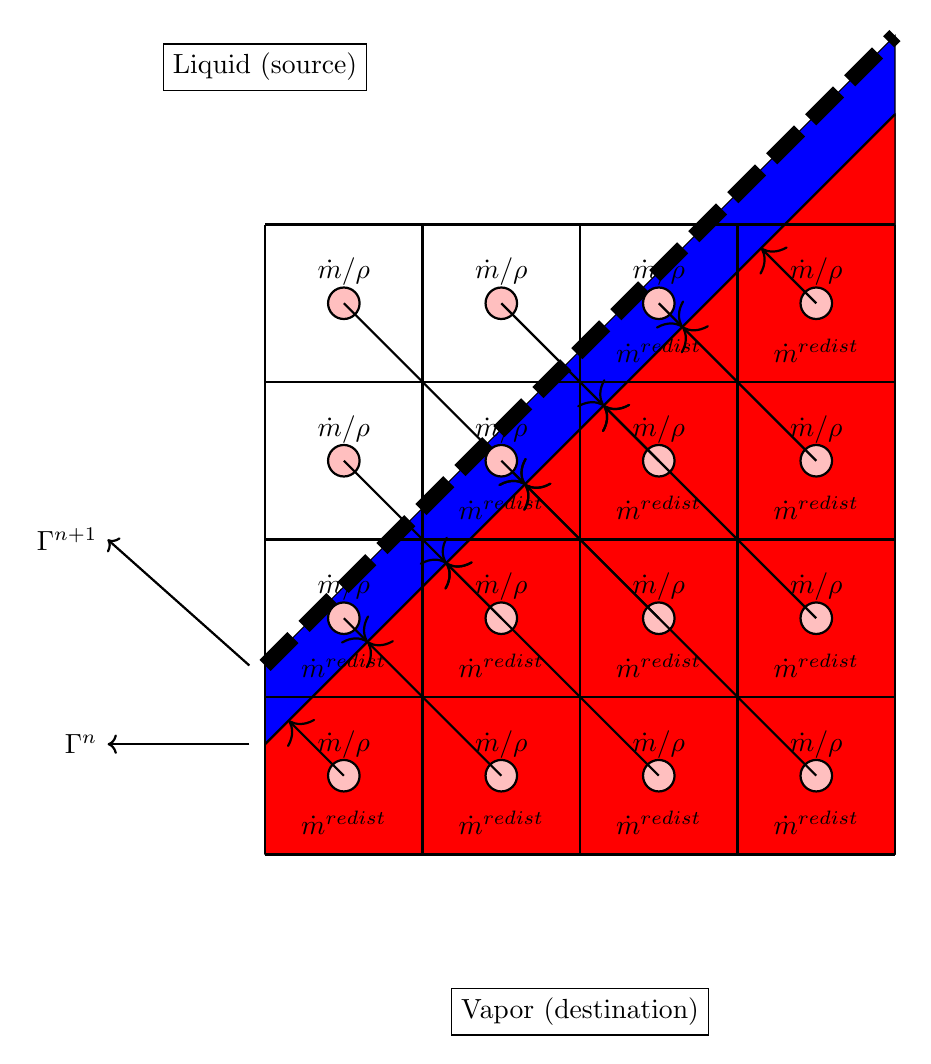
\begin{tikzpicture}[x=2cm,y=2cm]
\node[draw] at (0,5) {Liquid (source)};
\node[draw] at (2,-1.0) {Vapor (destination)};
\filldraw[draw=black,fill=blue] (0,0) -- (4,0) -- (4,5.2) -- (0,1.2) -- cycle;
\filldraw[draw=black,fill=red] (0,0) -- (4,0) -- (4,4.7) -- (0,0.7) -- cycle;
\draw[thick,black,->] (-0.1,1.2) -- (-1.0,2.0) node[left] {$\Gamma^{n+1}$};
\draw[line width=2mm,black,dash pattern=on 5mm off 2mm] (0,1.2) -- (4.0,5.2);
\draw[thick,black,->] (-0.1,0.7) -- (-1.0,0.7) node[left] {$\Gamma^{n}$};
\draw[thick,black] (0,0.7) -- (4,4.7);
\draw[step=1.0,black,thick] (0,0) grid (4,4);
\foreach \x in {0,...,3}
 \foreach \y in {0,1,2,3}
 {
  \filldraw[draw=black,fill=pink,thick] (\x+0.5,\y+0.5) circle (0.1);
  \pgfmathsetmacro{\xx}{(\x+\y+0.3)/2.0};
  \pgfmathsetmacro{\yy}{(\x+\y+1.7)/2.0};
  \pgfmathsetmacro{\ytest}{\x+1.2-\y};
  \tikzmath{
    if \ytest>0 then {
     \yinteger=1;
    } else {
     \yinteger=0;
    };
  }
  \draw[thick,black,-{>[scale=2.0,black]}] (\x+0.5,\y+0.5) -- (\xx,\yy);
  \node at (\x+0.5,\y+0.7) {$\dot{m}/\rho$};
  \ifthenelse{\yinteger>0}{
    \node at (\x+0.5,\y+0.2) {$\dot{m}^{redist}$};
  }{
   %%do nothing
  }
 }
\end{tikzpicture}
\caption{The phase change algorithm: (1) the phase change speed, 
$\dot{m}/\rho$, is approximated at all narrow band cells by evaluating
$\dot{m}/\rho$ at the corresponding closest point on the interface
($\Gamma^{n}$). (2) The change in volume fraction due to unsplit CISL
advection determines the mass source, $\dot{m}$, for the projection
step.  (3) the mass source, $\dot{m}$ is distributed to the vapor
side of the $\Gamma^{n+1}$ interface.  At the next time step, the
interface is advected using $\vec{u}^{source}$.  For compressible flow,
there is a problem if $\dot{m}$ is not distributed deep enough into
the vapor material.  This is because the corrector advection of 
$\Gamma^{n}$ will now have some redistributed $\dot{m}$ terms on the
liquid side of the $\Gamma_{n}$ interface (the blue region).
   \label{mdotproblem} }
\end{figure}

\section{Applications}

\begin{description}
	\item[1.] Jet in cross flow problem (military jet engines, Pratt
		and Whitney)
	\item[2.] Diesel injectors
	\item[3.] Rotating Detonation Engines (see latest article with Everett
		Wenzel and Marco Arienti).
\end{description}

\section{Algorithm}

\begin{description}
	\item[1.] Cell integrated semi Lagrangian advection
	\item[2.] Cell integrated semi Lagrangian advection due to phase 
		change.  
	\item[3.] Viscosity, Viscoelastic, and elastic forces.
	\item[4.] Temperature Diffusion
	\item[5.] Mass Fraction Diffusion
	\item[6.] Pressure Gradient
	\item[7.] Go back to step 1.
\end{description}

%%\biboptions{sort&compress}
\bibliography{cmof_paper}

\end{document}
%%% Local Variables:
%%% mode: latex
%%% TeX-master: t
%%% End:
